\chapter{مقدمه}
\label{chapter:introduction}

در این فصل به کلیت مسئله‌ی کدگذاری اندیس میپردازیم. با تاریخچه تحقیقاتی و کاربرها و اهمیت آن در صنعت و تعریف دقیق ان آشنا میشویم.
\pagebreak

\section{مقدمه}

کدگزاری اندیس در سال ۱۹۸۸ توسط در
\cite{ISCOD}
در هنگام بررسی ارتباطات ماهواره‌ای معرفی شد. از آن پس مسئله‌ی کدگذاری اندیس کاربردهای متعددی در مسائل مختلف نظری و عملی پیدا کرد. این موضوع باعث شده طی دو دهه گذشته ابزارهای مختلفی از بخش‌های مختلف ریاضی مانند نظریه گراف نظریه، نظریه کدگذاری و نظریه اطلاعات برای توسعه آن استفاده شوند.

	با وجود کاربردهای گوناگون این مسئله اما همان طور که در فصل دوم خواهیم دید این مسئله
\transf{ان‌پی-سخت}{NP-Hard}
است و در نتیجه امیدی به حل حالت کلی آن نیست. برای همین سویه‌های مختلفی برای آن توسعه داده شده است که هر کدام مدل یک مسئله‌ی دنیای واقعی هستند.

در این فصل ابتدا با تعریف مقدماتی مسئله کدگذاری اندیس و کاربردها و اهمیت آن آشنا میشویم سپس به تارخچه پژوهشی این موضوع پرداخته و در نهایت ساختار این پایان نامه را شرح میدهیم.

\section{تعریف مسئله}
مسئله را با یک مثال توضیح می‌دهیم. فرض کنید یک ماهواره‌‌ی رسانه‌ای در حال ارسال اطلاعات برای خبرنگار مختلف است. هر خبرنگار بسته به موقعیت مکانی خود و ارتباط دیگری که دارد از تعدادی از خبرهای روز مطلع است و به دنبال یک خبر جدید است که از آن اطلاعی ندارد تا برای مخاطب محلی خود بازگو کند. ماهواره در هر لحظه میتواند یکی از خبرهای روز را از طریق امواج به سمت کره‌ی زمین ارسال کند که در این صورت تمام خبرنگاران آن خبر را دریافت خواهند کرد. اگر خبرنگاری خبری را دریافت کند که از پیش میداند و یا به هر دلیلی به دنبال آن نیست باید صبر کند تا خبر مورد نظر خود را دریافت کند. مثلا در شکل زیر:
\centering
\begin{tikzpicture}[->, >=stealth, auto, semithick]
	% Set the positions of the nodes
	\alt<1,2,3,4>{
		\node[circle, draw=blue, fill=blue!20, inner sep=0pt] (P1) at (0,2) {
			
\includegraphics[width=0.07\linewidth]{img/hosseinmp76}
		};	
	}{
		\node[circle, draw=blue, fill=blue!20, inner sep=0pt] (P1) at (-3,2) {
			
\includegraphics[width=0.07\linewidth]{img/hosseinmp76}
		};
	}
	\alt<5->{\node[circle, draw=blue, fill=blue!20, inner sep=0pt] (P2) at (3,2) {
			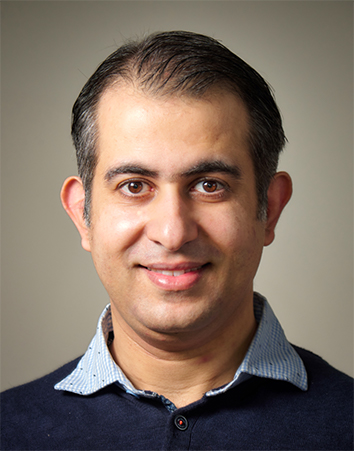
\includegraphics[width=0.06\linewidth]{img/javad}};
	}{}
	
	\alt<5->{\node[above] at (0,2.5) {people};}{}
	
	\alt<2-5>{
		\node[circle, draw=red, fill=red!20, inner sep=0pt] (M1) at (0,0) {
			
\includegraphics[width=0.07\linewidth]{img/fox}
			
		};
		\node[below] at (0,-0.75) {Fox News};
	}{}
	\alt<6->{
		\node[circle, draw=red, fill=red!20, inner sep=0pt] (M1) at (-6,0) {
			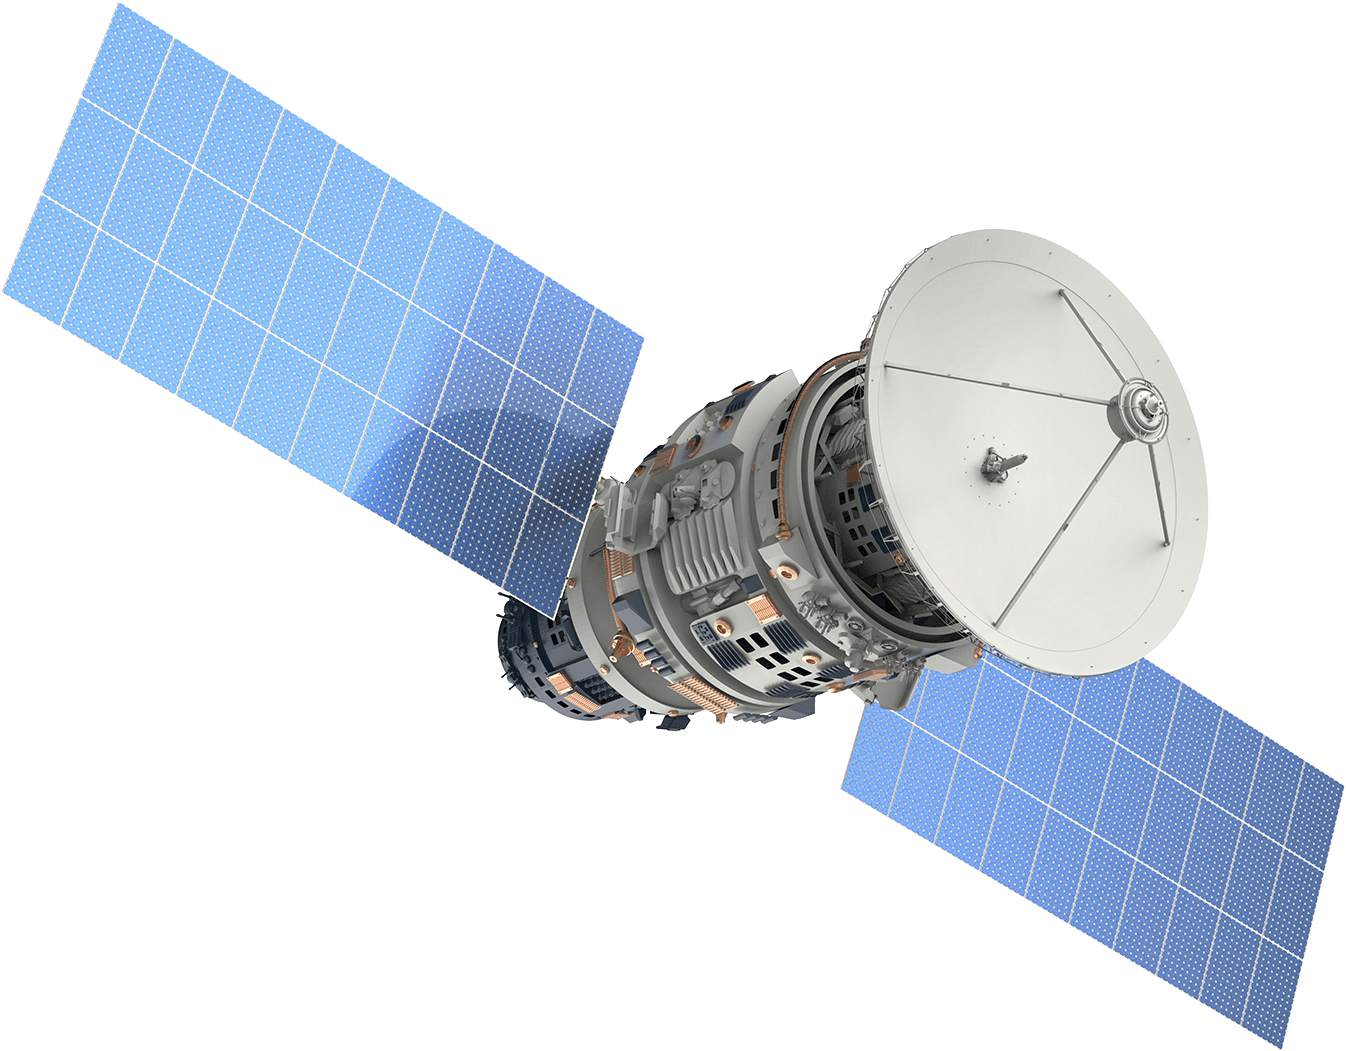
\includegraphics[width=0.07\linewidth]{img/satelite.png}
			
		};
		\node[below] at (0,-0.75) {Fox News};
	}{}
	\alt<3->{
		\node[circle, draw=green, fill=green!20, inner sep=0pt] (N1) at (-3,-2.5) {
			
\includegraphics[width=0.1\linewidth]{img/fox5}
			
			
		};
		\node[circle, draw=green, fill=green!20, inner sep=0pt] (N2) at (0,-2.5) {
			
\includegraphics[width=0.1\linewidth]{img/fox3}
			
		};
		\node[circle, draw=green, fill=green!20, inner sep=0pt] (N3) at (3,-2.5) {
			
\includegraphics[width=0.1\linewidth]{img/fox4}
			
		};
		\node[below] at (0,-3.5) {news };
	}{}
	
	\alt<2-5>{
		% Draw the edges
		\draw (P1) -- (M1);
	}{}
	\alt<3-5>{
		% Draw the edges
		\draw (M1) -- (N1) ;
		\draw (M1) -- (N2) ;
		\draw (M1) -- (N3) ;
	}{}
	\alt<5>{
		% Draw the edges
		\draw (P2) -- (M1);
	}{}
	\alt<4->{
		% Draw the edges
		\draw[->, color=red] (P1) -- (N1);
	}{}
	\alt<5->{
		% Draw the edges
		\draw[->, color=red] (P2) -- (N2);
		\draw[->, color=red] (P2) -- (N3);
	}{}
\end{tikzpicture}

 اگر خبرنگاران را با

و خبرها را با

نشان دهیم خبر نگار اول خبر دوم و سوم را میداند و به دنبال خبر اول است. به طور مشابه برای خبرنگاه دوم و سوم هم برقرار است.
کمترین تعداد دفعات ارسال خبر از طرف ماهواره برای اینکه تمام خبرنگاران به پیام مورد نظر خود دست بیابند چند است؟

اگر پیام ها را به چشم متغیرهای تصادفی در نظر بگیریم که از مجموعه‌ی مرجع

می‌آیند و هر ارسال ماهواره را برابر ارسال یک متغییر تصادفی بدانیم راه اول این است که ماهواره به ترتیب خبر مورد نظر هر خبرنگار را ارسال کند در این صورت به تعداد خبرنگران ارسال پیام نیاز داریم.
راه دیگر این است که ماهواره مقدار

را ارسال کند. در این صورت خبرنگار اول با استفاده از فرمول

میتواند خبر مورد نظر خود را دریافت کند. دو خبرنگار دیگر نیز به طور مشابه با همین تک ارسال میتوانند خبرمورد نظر خود را بیابند و در نتیجه تنها با یک ارسال به جای ۳ ارسال ماهواره می‌تواند تمام نیاز تمام خبرنگاران را رفع کند.

در واقع در مسئله‌ی کدگذاری اندیس
$m$
متغیر تصادفی و
$n$
کاربر داریم که هر کاربر به صورت اطلاعات جانبی(از پیش داشته) مقدار بعضی از متغیر ها را میداند و به دنبال مقدار یک متغیر تصادفی خاص است.

برای نمایش مسئله می‌توانیم از گارف‌های دوبخشی استفاده کنیم. به این صورت که در یک بخش رئوسی متناظر متغییر های تصادفی و در یک بخش رئوسی متناظر کاربرها میگذاریم. به ازای هر کاربری که یکی از متغییر ها را میداند یک یال بین رئوس متناظر از راس کاربر به راس متغییر میکشیم.



\section{اهمیت موضوع}

وجود قالب استاندارد برای نگارش پایان‌نامه از جهات مختلف حائز اهمیت است، از جمله:

\begin{itemize}
\item ایجاد یکنواختی در قالب کلی صفحات و شکل و اندازه‌ی قلم‌ها
\item تسهیل نگارش پایان‌نامه با در اختیار گذاشتن یک قالب اولیه
\item تولید خودکار صفحات دارای بخش‌های تکراری نظیر صفحات ابتدایی و انتهایی پایان‌نامه
\item پیش‌گیری از برخی خطاهای مرسوم در نگارش پایان‌نامه
\end{itemize}

\section{ادبیات موضوع}

اکثر دانشگاه‌های معتبر قالب استانداردی برای تهیه‌ی پایان‌نامه در اختیار دانشجویان خود قرار می‌دهند.
این قالب‌ها عموما مبتنی بر نرم‌افزارهای متداول حروف‌چینی نظیر لاتک و مایکروسافت ورد هستند.

 لاتک
 \LTRfootnote{\LaTeX}
  یک نرم‌افزار متن‌باز قوی برای حروفچینی متون علمی است.\cite
 {knuth1984texbook, lamport1985LaTeX}
در این نوشتار از نرم‌افزار حروف‌چینی زی‌تک
\LTRfootnote{\XeTeX}
 و افزونه‌ی زی‌پرشین
 \LTRfootnote{\XePersian}
 استفاده شده است.


\section{اهداف پژوهش}

دانشگاه صنعتی شریف دستورالعمل جامعی را در خصوص
نحوه تهیه پایان‌نامه کارشناسی ارشد و رساله دکتری توسط کتابخانه مرکزی دانشگاه ارائه کرده است.
در این نوشتار سعی شده است قالب استانداردی برای تهیه‌ی پایان‌نامه‌ها مبتنی بر نرم‌افزار لاتک و
بر اساس دستورالعمل مذکور ارائه شده و
نحوه‌ی استفاده از قالب به طور مختصر توضیح داده شود.
این قالب  می‌تواند برای تهیه‌ی پایان‌نامه‌های کارشناسی و کارشناسی ارشد
و همجنین رساله‌ها‌ی دکتری مورد استفاده قرار گیرد.

\section{ساختار پایان‌نامه}

این پایان‌نامه در پنج فصل به شرح زیر ارائه می‌شود.
%فصل دوم به بیان مفاهیم اولیه  می‌پردازد.
نکات اولیه نگارشی و نحوه‌ی نگارش پایان‌نامه در محیط لاتک در  فصل دوم به اختصار اشاره شده است.
فصل سوم به مطالعه و بررسی کارهای پیشین مرتبط با موضوع این پایان‌نامه می‌پردازد.
در فصل چهارم، نتایج جدیدی که در این پایان‌نامه به‌دست آمده است، ارائه می‌شود.
فصل پنجم به جمع‌بندی کارهای انجام شده در این پژوهش و ارائه‌ی پیشنهادهایی برای انجام کارهای آتی خواهد پرداخت.